\documentclass[tikz,border=2pt]{standalone}
\usepackage{pgfplots}
\pgfplotsset{compat=newest}

\begin{document}
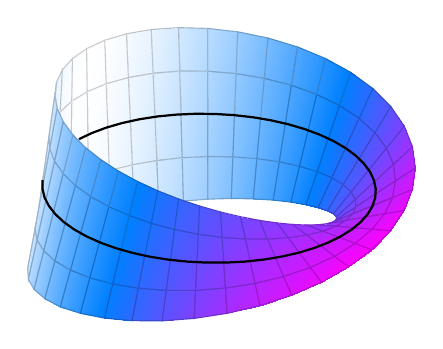
\begin{tikzpicture}
\begin{axis}[hide axis, view={40}{40}]
  \addplot3[
    surf, colormap/cool, shader=faceted interp,
    point meta=x, samples=40, samples y=5,
    z buffer=sort, domain=0:360, y domain=-0.5:0.5
  ] (
    {(1+0.5*y*cos(x/2))*cos(x)},
    {(1+0.5*y*cos(x/2))*sin(x)},
    {0.5*y*sin(x/2)}
  );
  \addplot3[samples=50, domain=-145:180, samples y=0, thick]
    ({cos(x)},{sin(x)},{0});
\end{axis}
\end{tikzpicture}
\end{document}
